% This template was created by H. Huegel

%\documentclass{tuhhproc-en}
\documentclass[12pt,twoside]{tuhhproc-en}
\usepackage[latin1]{inputenc}
\usepackage[T1]{fontenc}
\usepackage{times,rotating}

\usepackage[backend=biber, style=numeric, citestyle=authoryear, sorting=nty, natbib=true]{biblatex}
\bibliography{references} %Location of references.bib only for biblatex

%%%%%%%%%%%%%%%%%%%%%%%%%%%%%%%%%%%%%%%%%%%%%%%%%%%%%%%%%%%%%%%%%%%%%%%%%%
\usepackage{cleveref}
\usepackage{dsfont}
\RequirePackage{amsmath,amsfonts,amssymb}
\RequirePackage{booktabs}

\usepackage[per=slash]{siunitx} % use this package module for SI units
\usepackage{subcaption}

\selectlanguage{english}
\pagenumbering{gobble}

\begin{document}
\selectlanguage{english}

\Header{Granular column collapse on slope: Effect of permeability on the runout characteristics}{Krishna Kumar, Jean-Yves Delenne, Kenichi Soga}{1}

\Abstract{This paper investigates the effect of permeability on the runout characteristics of collapse of  granular columns on slopes in fluid. Two-dimensional sub-grain scale numerical simulations are performed to understand the flow dynamics of granular collapse in fluid. The Discrete Element (DEM) technique is coupled with the Lattice Boltzmann Method (LBM), for fluid-grain interactions, to understand the evolution of submerged granular flows. The fluid phase is simulated using Multiple-Relaxation-Time LBM (LBM-MRT) for numerical stability. In order to simulate interconnected pore space in 2D, a reduction in the radius of the grains (hydrodynamic radius) is assumed during LBM computations. The collapse of granular column in fluid is compared with the dry cases to understand the effect of fluid on the runout behaviour. A parametric analysis is performed to assess the influence of the granular characteristics (initial packing) on the evolution of flow and run-out distances for slope angles of 5°. In order to understand the effect of permeability on granular flow down a slope angle of 5°, the collapse of a granular column with an initial aspect ratio of 0.8 is simulated with different permeabilities. The hydrodynamic radius of a loosely packed granular column is varied from r = 0.7 R (high permeability), 0.75 R, 0.8 R, 0.85 R to 0.9 R (low permeability). The granular flow dynamics is investigated by analysing the effect of hydroplaning, water entrainment and viscous drag on the granular mass. The mechanism of energy dissipation, shape of the flow front, water entrainment and evolution of packing density is used to explain the difference in the flow characteristics of granular column collapse in fluid.}

\section{Introduction}
Catastrophic earth movement events, such as landslides, debris flows, rock avalanches and reservoir embankment failures, exemplify the potential consequences of an earth gravitational instability. Slope failure is a problem of high practical importance for both civil engineering structures and natural hazard management. The study described in this paper examines the stability of underwater slopes, which are caused by excess seepage or earthquakes.  They can damage offshore structures nearby and may generate a tsunami. 

In order to describe the mechanism of underwater granular flows, it is necessary to consider both the dynamics of the solid phase of granular matter and the role of the ambient fluid, which exists either inside the pores of the granular body and as free water outside the granular body~\citep{Denlinger2001,Iverson1997}. Initial acceleration plays a crucial role in underwater landslide propagation~\citep{Romano2017}, as the initial acceleration increases, there is a limited time for the landslide to deform during the acceleration phase. The initiation and propagation of submarine granular flows depend mainly on geometry (e.g. slope angle, lateral extent, etc), initial stress conditions, density, soil properties, and the quantity of the material destabilised. Although certain macroscopic models are capable of capturing simple mechanical behaviour (e.g.~\citet{Topin2011}), the complex fundamental mechanism that occurs at the grain scale, such as hydrodynamic instabilities, the formation of clusters, collapse, and transport, require further investigation in order to make better engineering assessment of the potential risk of damages against underwater slope failures for example. 

The momentum transfer between the discrete and the continuous phases of fluid saturated granular material significantly affects the dynamics of the flow~\citep{Peker2007}.
The grain-scale description of the granular material enriches the macro-scale variables. In particular, when the solid phase reaches a high-volume fraction, it is important to consider the strong heterogeneity arising from the contact forces between the grains, the drag interactions which counteract the movement of the grains, and the hydrodynamic forces that reduce the weight of the grains inducing a transition from a dense compacted to a dense suspended flow~\citep{Meruane2010}. 

The case of granular material movements in presence of an interstitial fluid at the grain-scale has been less studied. In this paper, we report the findings of the study on the granular column collapse in fluid in the inclined configuration using the coupled Lattice Boltzmann Method (LBM) and Discrete Element Method (DEM). We examined the effect of density and slope angle on the runout evolution.


The Lattice Boltzmann Method is a `micro-particle' based numerical time-stepping procedure for the solution of incompressible fluid flows. Consider a 2D incompressible fluid flow with density $\rho$ and kinematic viscosity \textit{v}, in a rectangular domain \textit{\textbf{D}}. The fluid domain is divided into a rectangular grid or lattice, with the same spacing \textit{`h'} in both the \textit{x-} and the \textit{y-}directions, as shown in~\cref{fig:D2Q9}. The present study focuses on two-dimensional problems, hence the \textit{D2Q9} momentum discretisation is adopted (see \citep{He1997} for naming convention).

\begin{figure}[htpb]
\centering
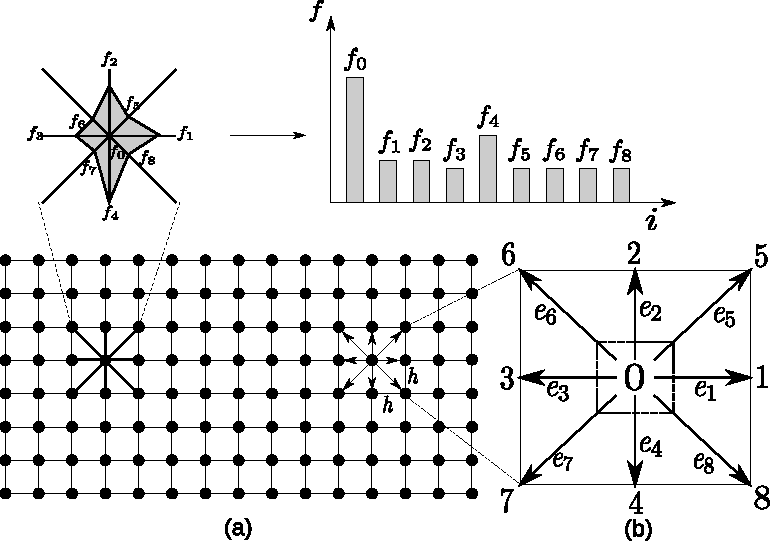
\includegraphics[width=0.45\textwidth]{figs/d2q9.pdf}
\caption[The Lattice Boltzmann discretisation and D2Q9 scheme]{The Lattice Boltzmann discretisation and D2Q9 scheme: (a) a standard LB lattice and histogram views of the discrete single particle distribution function/direction-specific densities $f_i$; (b) D2Q9 model}
\label{fig:D2Q9}
\end{figure}

The lattice Boltzmann Bhatnagar-Gross-Krook (LGBK) method is capable of simulating various hydrodynamics~\citep{Succi2001} and offers intrinsic parallelism. Although LBM is successful in modelling complex fluid systems, such as multiphase flows and suspensions in fluid, the LBM may lead to numerical instability when the dimensionless relaxation time $\tau$ is close to 0.5. The Multi-Relaxation Time Lattice Boltzmann Method (LBM-MRT) overcomes the deficiencies of linearlised single relaxation LBM-BGK, such as fixed Prandtl number (Pr=$\nu/\kappa$), where the thermal conductivity `$\kappa$' is unity~\citep{Liu2003a}. The LB-MRT model offers better numerical stability and has more degrees of freedom. In the formulation of the linear Boltzmann equation with multiple relaxation time approximation, the lattice Boltzmann equation is written as:

\begin{align}
&f_{\alpha}(\mathbf{x}+\mathbf{e}_i\Delta_t, t+ \Delta_t)-f_{\alpha}(\mathbf{x},t) \nonumber \\
&\mbox{\qquad\qquad} = -\mathbf{S}_{\alpha i}(f_i(\mathbf{x},t)-f_i^{eq}(\mathbf{x},t)
\end{align}

\noindent where \textbf{S} is collision matrix. The nine eigen values of \textbf{S} are all between 0 and 2 so as to maintain linear stability and the separation of scales, which means that the relaxation times of non-conserved quantities are much faster than the hydrodynamic time scales. The LGBK model is the special case in which the nine relaxation times are all equal and the collision matrix $\mathbf{S}=\frac{1}{\tau}\mathbf{I}$, where \textbf{I} is the identity matrix. The evolutionary progress involves two steps, advection and flux. The advection can be mapped to the momentum space by multiplying through by a transformation matrix \textbf{M} and the flux is still finished in the velocity space. The evolutionary equation of the multi-relaxation time lattice Boltzmann equation is written as:

\begin{align}
&\mathbf{f}(\mathbf{x}+\mathbf{e}_i\Delta_t, t+ \Delta_t)-\mathbf{f}(\mathbf{x},t) \nonumber \\
&\mbox{\qquad\qquad} = -M^{-1}\hat{\mathbf{S}} (\hat{\mathbf{f}}(\mathbf{x},t)-\hat{\mathbf{f}}^{eq}(\mathbf{x},t))
\end{align}

\noindent where \textbf{M} is the transformation matrix mapping a vector \textbf{f} in the discrete velocity space $\mathds{V}=\mathds{R}^b$ to a vector $\hat{\mathbf{f}}$ in the moment space $\mathds{V}=\mathds{R}^b$.

\begin{align}
&\hat{\mathbf{f}} = \mathbf{M}\mathbf{f}\\
&\mathbf{f}(\mathbf{x},t) = \left[f_0(\mathbf{x},t),f_1(\mathbf{x},t),\dots f_8(\mathbf{x},t)\right]^T
\end{align}

The collision matrix $\hat{\mathbf{S}} = MSM^{-1}$ in moment space is a diagonal matrix: $\hat{\mathbf{S}} =\mbox{diag} \left[ s_1, s_2, s_3,\dots s_9  \right]$. The transformation matrix \textbf{M} can be constructed via Gram-Schmidt orthgonalisation procedure. Through the Chapman-Enskog expansion~\citep{Du2006}, the incompressible Navier-Stokes equation can be recovered and the viscosity is given as:
\begin{align}
\nu=c_s^2\Delta t(\tau-0.5)
\end{align}


\subsection{Turbulence in Lattice Boltzmann Method}
Modelling fluids with low viscosity like water remains a challenge, necessitating very small values of \textit{h}, and/or $\tau$ very close to 0.5~\citep{He1997}. Turbulent flows are characterised by the occurrence of eddies with multiple scales in space, time and energy. In this study, the Large Eddy Simulation (LES) is adopted to solve for turbulent flow problems. The separation of scales is achieved by filtering of the Navier-Stokes equations, from which the resolved scales are directly obtained and unresolved scales are modelled by a one-parameter Smagorinski sub-grid methodology, which assumes that the Reynold's stress tensor is dependent only on the local strain rate~\citep{Smagorinsky1963}. The turbulent viscosity $\nu$ is related to the strain rate $S_{ij}$ and a filtered length scale `h' as follows:
\begin{align}
&\mathit{v}_{\mathit{t}}  =  (\mathit{S}_{c}\mathit{h})^{2}\overline{S}; \\
&\overline{S}  = \sqrt{\sum\limits_{\mathit{i,j}}{\tilde{S}_{\mathit{i,j}}\tilde{S}_{\mathit{i,j}}}}
\end{align}
where $\mathit{S}_{c}$ is the Smagorinski constant found to be close to 0.03~\citep{Yu2005}.

The effect of the unresolved scale motion is taken into account by introducing an effective collision relaxation time scale $\tau_{t}$, so that the total relaxation time $\tau_{*}$ is written as:
\begin{align}
\tau_{*}=\tau + \tau_{t}
\end{align}
where $\tau$ and $\tau_{t}$ are respectively the standard relaxation times corresponding to the true fluid viscosity \textit{v} and the turbulence viscosity $\mathit{v}_{\mathit{t}}$, defined by a sub-grid turbulence model. The new viscosity $\mathit{v}_{*}$ corresponding to $\tau_{*}$ is defined as:
\begin{align}
& \mathit{v}_{*}=\mathit{v}+\mathit{v}_{\mathit{t}}=\frac{1}{3}(\tau+\tau_{t}-\frac{1}{2})\mathit{C}^{2} \Delta \mathit{t}  \\
& \mathit{v}_{\mathit{t}}=\frac{1}{3}\tau_{\mathit{t}}\mathit{C}^{2} \Delta \textit{t}
\end{align}
The Smagorinski model is easy to implement and the Lattice Boltzmann formulation remains unchanged, except for the use of a new turbulence-related viscosity $\tau_{*}$. The component $s_1$ of the collision matrix becomes $s_1 = \frac{1}{\tau+\tau_t}$.


\section{Coupled LB-DEM model}
\subsection{General}
The Lattice Boltzmann approach has the advantage of accommodating large particle sizes and the interaction between the fluid and the moving particles can be modelled through relatively simple fluid - particle interface treatments. Further, employing the Discrete Element Method (DEM) to account for the particle/particle interaction naturally leads to a combined LB - DEM solution procedure. The Eulerian nature of the Lattice Boltzmann formulation, together with the common explicit time step scheme of both the Lattice Boltzmann and the Discrete Element, makes this coupling strategy an efficient numerical procedure for the simulation of particle-fluid systems~\citep{Cook2004}. The LB-DEM coupling system is a powerful fundamental research tool for investigating hydro-mechanical physics in porous media flow~\citep{Han2013}. To capture the actual physical behaviour of a fluid-particle system, the boundary condition between the fluid and the particle is modelled as a non-slip boundary condition, i.e. the fluid near the particle should have a similar velocity as the particle boundary. The solid particles inside the fluid are represented as solid lattice nodes. The discrete nature of lattice will result in stepwise representation of the surfaces~\citep{Kumar2015}. A very small lattice spacing is adopted to obtain smoother boundaries.

The smallest DEM grain in the system controls the size of the lattice. In the present study, a very fine resolution of $d_{min}/h = 10$ is adopted. That is, the smallest grain with a diameter dmin in the system is discretized into 100 lattice nodes ($10h \times 10h$). This provides a very accurate representation of the interaction between the solid and the fluid nodes. 

When combining the Discrete Element modelling of grain interactions with the lattice Boltzmann formulation, an issue arises. That is, there are now two time steps: $\Delta t$ for the fluid flow and $\Delta t_D$ for the particle movements. Since $\Delta t_D$ is normally smaller than $\Delta t$, $\Delta t_D$ is slightly reduced to a new value $\Delta t_s$ so that $\Delta t$ and $\Delta t_s$ have an integer ratio $n_s$:

\begin{align}
  \Delta t_s = & \Delta t / n_s \\
  n_s  = & [\Delta t/\Delta t_D]+1
\end{align}

This results in a subcycling time integration for the Discrete Element part.  $\Delta t$ every step of the fluid computation, $n_s$ sub-steps of integration are performed for DEM using the time step  $\Delta t_s$. The hydrodynamic force is unchanged during this sub-cycling.

\selectlanguage{english}
\section*{References}
\printbibliography[heading=none]

\section*{Author}\small
Dr.\ Krishna Kumar\\
Department of Engineering \\
University of Cambridge \\
Cambridge, CB2 1PZ\\
Tel.: +44(0) 1223 748 589\\
e-mail: \url{kks32@cam.ac.uk}\\
Web: \url{www.cb-geo.com}\\

\end{document}
